\setcounter{section}{33}
\section{Алгоритм dfs на неориентированном графе. Дерево обхода dfs. Классификация рёбер на древесные и обратные. Проверка связности и ацикличности. Компоненты связности}
В отличие от ориентированного графа, в неориентированном не будет ребер в черные вершины, поскольку на графе нет ориентации. Когда мы обходим граф, у нас могут быть только  ребра в серые вершины.
\begin{center}
    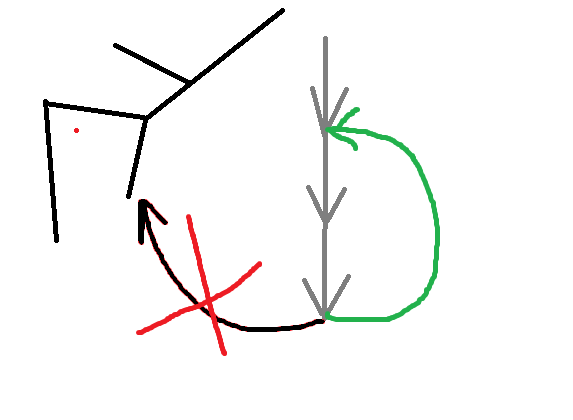
\includegraphics[width=7cm]{images/34_alg17.PNG}
\end{center}
Это - дерево dfs. Ребра, идущие в порядке обхода dfs будем называть \textit{древесные ребра}, а те, что не были посещены dfs(они вели в серые вершины) - \textit{обратные}
\begin{verbatim}
vector<vector<int>> g;
vector<bool> used;

void dfs(int v, int p = -1){
    used[v] = true;
    for(int to: g[v]){
        if(!used[to]) 
            dfs(to,v)
    }
}
\end{verbatim}

\textbf{Проверка на связность} \\
Выберем какую-нибудь вершину в графе, запустим dfs из нее и проверим, что dfs обошел все вершины графа
\\
\\
\textbf{Проверка на ацикличность} \\
Будем искать цикл почти так же, как и в ориентированном случае, но теперь нас интересует ребро не в серую вершину, а в любую использованную, не являющуюся непосредственным родителем текущей
\\
\\
Введем отношение $\sim$ . u $\sim$ v, если между вершинами u и v есть путь. Очевидно, это отношение является отношением эквивалентности\\
Тогда граф распадается на классы эквивалентности, называемые \textit{компонентами связности} \\ 
\textbf{Определение} \textit{Компонента связности графа} G (или просто компонента графа G) — максимальный (по включению) связный подграф графа G.
\begin{center}
    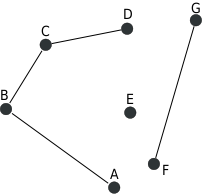
\includegraphics[width=5cm]{images/34_alg18.png}
\end{center} Здесь 3 компоненты связности